\documentclass{article}
\usepackage{amsmath,amssymb,amsthm,graphicx,setspace,fullpage,verbatim,listings,xcolor}

\onehalfspace 

\title{\bf\huge AI+X: Report 3}
\author{Hanxi Lin}

\lstset{
	backgroundcolor=\color{gray!10},   % 背景色
	basicstyle=\ttfamily\footnotesize, % 基本字体样式
	breaklines=true,                  % 自动换行
	frame=noframe,                     % 边框样式
	numbers=left,                     % 行号位置
	numberstyle=\tiny\color{gray},    % 行号样式
	keywordstyle=\color{blue},        % 关键字样式
	commentstyle=\color{green!50!black}, % 注释样式
	stringstyle=\color{orange},       % 字符串样式
	showstringspaces=false            % 不显示字符串中的空格
}

\begin{document}
\maketitle

\begin{figure}[h]
    \centering
    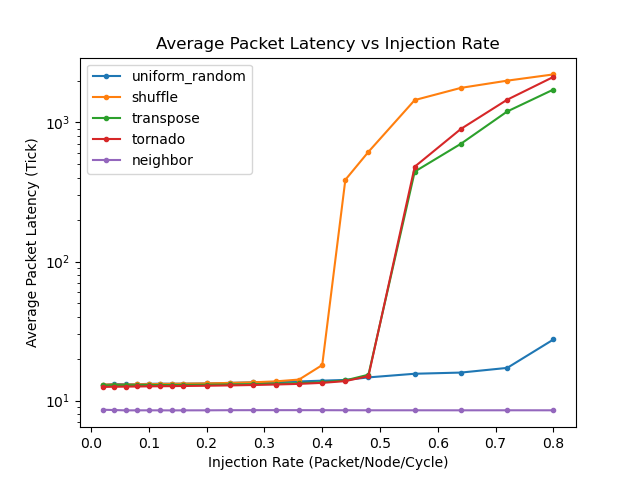
\includegraphics[width=0.49\textwidth]{lab3-SYNTHETIC_TRAFFIC.png}
    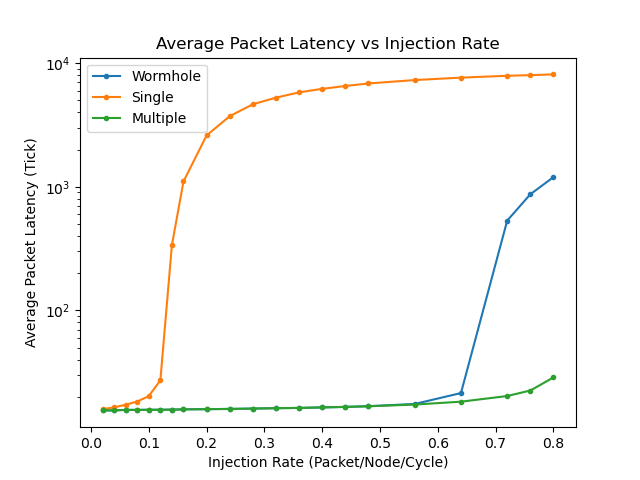
\includegraphics[width=0.49\textwidth]{lab3-VC_TYPE.png}
    \caption{Average packet latency vs. injection rate}
\end{figure}

\section*{Task 1}
We've implemented a simple minimal routing algorithm for a ring topology (which is not deadlock-free). As shown in figure, structured synthetic traffics such as tornado are more likely to cause deadlocks, hence lower congestion points.

\section*{Task 2}
As shown in figure, using wormhole far improves the performance of a single virtual channel. However, wormhole doesn't perform as well as the same capacity of virtual channels. This is because wormhole requires all flits in a packet to be sent in order, which may cause blocking if the head flit is blocked. On the other hand, virtual channels can send flits from different packets in an interleaved manner, which improves the overall throughput.

An interesting observation: wormhole performs as well as 4 virtual channels.

\section*{Appendix}
\begin{lstlisting}[language=bash]
#! /bin/bash

NUM_CPUS=16
SIM_CYCLES=10000

echo > network_stats.txt

for SYNTH in uniform_random 
do
	echo "SYNTHETIC TRAFFIC: $SYNTH" >> network_stats.txt
	for INJ_RATE in 0.02 0.04 0.06 0.08 0.10 0.12 0.14 0.16 0.20 0.24 0.28 0.32 0.40 0.48 0.56 0.64 0.72 0.80
	do
		./build/NULL/gem5.opt \
		configs/example/garnet_synth_traffic.py \
		--network=garnet --num-cpus=$NUM_CPUS --num-dirs=64 \
		--topology=Ring --routing-algorithm=3\
		--inj-vnet=0 --vcs-per-vnet=2 --synthetic=$SYNTH \
		--sim-cycles=$SIM_CYCLES --injectionrate=$INJ_RATE
		INJ_TOT=$(grep -Eo "packets_injected::total\s*[0-9.]*" m5out/stats.txt | grep -Eo "[0-9.]*")
		RECV_TOT=$(grep -Eo "packets_received::total\s*[0-9.]*" m5out/stats.txt | grep -Eo "[0-9.]*")
		RECV_RATE=$(echo "scale=6;$RECV_TOT/$NUM_CPUS/$SIM_CYCLES" | bc)
		AVG_PKT_QUEUE_LATENCY=$(grep -Eo "average_packet_queueing_latency\s*[0-9.]*" m5out/stats.txt | grep -Eo "[0-9.]*")
		AVG_PKT_NETWK_LATENCY=$(grep -Eo "average_packet_network_latency\s*[0-9.]*" m5out/stats.txt | grep -Eo "[0-9.]*")
		AVG_PKT_LATENCY=$(grep -Eo "average_packet_latency\s*[0-9.]*" m5out/stats.txt | grep -Eo "[0-9.]*")
		AVG_HOPS=$(grep -Eo "average_hops\s*[0-9.]*" m5out/stats.txt | grep -Eo "[0-9.]*")
		echo "[$INJ_RATE, $INJ_TOT, $RECV_TOT, $RECV_RATE, $AVG_PKT_QUEUE_LATENCY, $AVG_PKT_NETWK_LATENCY, $AVG_PKT_LATENCY, $AVG_HOPS]" >> network_stats.txt
	done
	echo >> network_stats.txt
done

python3 plot.py

NUM_CPUS=64

echo > network_stats.txt
echo "VC TYPE: Wormhole" >> network_stats.txt
for INJ_RATE in 0.02 0.04 0.06 0.08 0.10 0.12 0.14 0.16 0.20 0.24 0.28 0.32 0.40 0.48 0.56 0.64 0.72 0.80
	do
		./build/NULL/gem5.opt \
		configs/example/garnet_synth_traffic.py \
		--network=garnet --num-cpus=$NUM_CPUS --num-dirs=64 \
		--topology=Mesh_XY --mesh-rows=8 \
		--inj-vnet=0 --synthetic=uniform_random \
		--sim-cycles=$SIM_CYCLES --injectionrate=$INJ_RATE --wormhole
		INJ_TOT=$(grep -Eo "packets_injected::total\s*[0-9.]*" m5out/stats.txt | grep -Eo "[0-9.]*")
		RECV_TOT=$(grep -Eo "packets_received::total\s*[0-9.]*" m5out/stats.txt | grep -Eo "[0-9.]*")
		RECV_RATE=$(echo "scale=6;$RECV_TOT/$NUM_CPUS/$SIM_CYCLES" | bc)
		AVG_PKT_QUEUE_LATENCY=$(grep -Eo "average_packet_queueing_latency\s*[0-9.]*" m5out/stats.txt | grep -Eo "[0-9.]*")
		AVG_PKT_NETWK_LATENCY=$(grep -Eo "average_packet_network_latency\s*[0-9.]*" m5out/stats.txt | grep -Eo "[0-9.]*")
		AVG_PKT_LATENCY=$(grep -Eo "average_packet_latency\s*[0-9.]*" m5out/stats.txt | grep -Eo "[0-9.]*")
		AVG_HOPS=$(grep -Eo "average_hops\s*[0-9.]*" m5out/stats.txt | grep -Eo "[0-9.]*")
		echo "[$INJ_RATE, $INJ_TOT, $RECV_TOT, $RECV_RATE, $AVG_PKT_QUEUE_LATENCY, $AVG_PKT_NETWK_LATENCY, $AVG_PKT_LATENCY, $AVG_HOPS]" >> network_stats.txt
	done
	echo >> network_stats.txt


echo "VC TYPE: Single" >> network_stats.txt
for INJ_RATE in 0.02 0.04 0.06 0.08 0.10 0.12 0.14 0.16 0.20 0.24 0.28 0.32 0.40 0.48 0.56 0.64 0.72 0.80
	do
		./build/NULL/gem5.opt \
		configs/example/garnet_synth_traffic.py \
		--network=garnet --num-cpus=$NUM_CPUS --num-dirs=64 \
		--topology=Mesh_XY --mesh-rows=8 \
		--inj-vnet=0 --synthetic=uniform_random \
		--sim-cycles=$SIM_CYCLES --injectionrate=$INJ_RATE --vcs-per-vnet=1
		INJ_TOT=$(grep -Eo "packets_injected::total\s*[0-9.]*" m5out/stats.txt | grep -Eo "[0-9.]*")
		RECV_TOT=$(grep -Eo "packets_received::total\s*[0-9.]*" m5out/stats.txt | grep -Eo "[0-9.]*")
		RECV_RATE=$(echo "scale=6;$RECV_TOT/$NUM_CPUS/$SIM_CYCLES" | bc)
		AVG_PKT_QUEUE_LATENCY=$(grep -Eo "average_packet_queueing_latency\s*[0-9.]*" m5out/stats.txt | grep -Eo "[0-9.]*")
		AVG_PKT_NETWK_LATENCY=$(grep -Eo "average_packet_network_latency\s*[0-9.]*" m5out/stats.txt | grep -Eo "[0-9.]*")
		AVG_PKT_LATENCY=$(grep -Eo "average_packet_latency\s*[0-9.]*" m5out/stats.txt | grep -Eo "[0-9.]*")
		AVG_HOPS=$(grep -Eo "average_hops\s*[0-9.]*" m5out/stats.txt | grep -Eo "[0-9.]*")
		echo "[$INJ_RATE, $INJ_TOT, $RECV_TOT, $RECV_RATE, $AVG_PKT_QUEUE_LATENCY, $AVG_PKT_NETWK_LATENCY, $AVG_PKT_LATENCY, $AVG_HOPS]" >> network_stats.txt
	done
	echo >> network_stats.txt


echo "VC TYPE: Multiple" >> network_stats.txt
for INJ_RATE in 0.02 0.04 0.06 0.08 0.10 0.12 0.14 0.16 0.20 0.24 0.28 0.32 0.40 0.48 0.56 0.64 0.72 0.80
	do
		./build/NULL/gem5.opt \
		configs/example/garnet_synth_traffic.py \
		--network=garnet --num-cpus=$NUM_CPUS --num-dirs=64 \
		--topology=Mesh_XY --mesh-rows=8 \
		--inj-vnet=0 --synthetic=uniform_random \
		--sim-cycles=$SIM_CYCLES --injectionrate=$INJ_RATE --vcs-per-vnet=16
		INJ_TOT=$(grep -Eo "packets_injected::total\s*[0-9.]*" m5out/stats.txt | grep -Eo "[0-9.]*")
		RECV_TOT=$(grep -Eo "packets_received::total\s*[0-9.]*" m5out/stats.txt | grep -Eo "[0-9.]*")
		RECV_RATE=$(echo "scale=6;$RECV_TOT/$NUM_CPUS/$SIM_CYCLES" | bc)
		AVG_PKT_QUEUE_LATENCY=$(grep -Eo "average_packet_queueing_latency\s*[0-9.]*" m5out/stats.txt | grep -Eo "[0-9.]*")
		AVG_PKT_NETWK_LATENCY=$(grep -Eo "average_packet_network_latency\s*[0-9.]*" m5out/stats.txt | grep -Eo "[0-9.]*")
		AVG_PKT_LATENCY=$(grep -Eo "average_packet_latency\s*[0-9.]*" m5out/stats.txt | grep -Eo "[0-9.]*")
		AVG_HOPS=$(grep -Eo "average_hops\s*[0-9.]*" m5out/stats.txt | grep -Eo "[0-9.]*")
		echo "[$INJ_RATE, $INJ_TOT, $RECV_TOT, $RECV_RATE, $AVG_PKT_QUEUE_LATENCY, $AVG_PKT_NETWK_LATENCY, $AVG_PKT_LATENCY, $AVG_HOPS]" >> network_stats.txt
	done
	echo >> network_stats.txt

python3 plot.py
\end{lstlisting}


\end{document}